\documentclass[nobib]{tufte-handout}
% \documentclass[fleqn,reqno,12pt]{article}

%========================================
% Packages
%========================================

\usepackage[nographicx, nohyperref, nosubcaption, nogb4e]{mfpackages}
\usepackage{subcaption}
\usepackage{mfenvironments}
\usepackage{mfcommands}
% for info boxes
\usepackage{newfloat, caption}
\DeclareCaptionType{InfoBox}
% for table spacing
\usepackage{array, booktabs}
\usepackage{tabularray}

\usepackage{float}
\usepackage{amsmath}
\usepackage{amssymb}
\usepackage{changepage}



%========================================
% Section numbering (in the left margin)
%========================================

\setcounter{secnumdepth}{5}
\renewcommand\thesection{\arabic{section}}

% this length controls tha hanging indent for titles
% change the value according to your needs
\newlength\titleindent
\setlength\titleindent{0.7cm}

% \pretocmd{\paragraph}{\stepcounter{subsection}}{}{}
% \pretocmd{\subparagraph}{\stepcounter{subsubsection}}{}{}

\titleformat{\chapter}[block]
  {\normalfont\huge\bfseries}{}{0pt}{\hspace*{-\titleindent}}

\titleformat{\section}
  {\normalfont\Large\itshape}{\llap{\parbox{\titleindent}{\thesection\hfill}}}{0em}{}

\titleformat{\subsection}
  {\normalfont\itshape}{\llap{\parbox{\titleindent}{\thesubsection\hfill}}}{0em}{}

\titleformat{\subsubsection}
  {\normalfont\normalsize\itshape}{\llap{\parbox{\titleindent}{\thesubsubsection}}}{0em}{}

% \titleformat{\paragraph}[runin]
%   {\normalfont\normalsize\itshape}{}{-0.7cm}{}[\xspace \ \ \ \ ]

\titleformat{\paragraph}[runin]
  {\normalfont\normalsize\itshape}{}{-0cm}{}[\xspace \ \ \ \ ]

\titleformat{\subparagraph}[runin]
  {\normalfont\normalsize}{\llap{\parbox{\titleindent}{\thesubsubsection\hfill}}}{0em}{}

\titlespacing*{\chapter}{0pt}{0pt}{20pt}
\titlespacing*{\subsubsection}{0pt}{3.25ex plus 1ex minus .2ex}{1.5ex plus .2ex}
\titlespacing*{\paragraph}{0pt}{3.25ex plus 1ex minus .2ex}{0em}
\titlespacing*{\subparagraph}{0pt}{3.25ex plus 1ex minus .2ex}{0em}



%========================================
% Bibliography
%========================================

\bibliography{references.bib}

%========================================
% General Layout Tweaks
%========================================

% \usepackage[margin=2cm]{geometry}

% Itemize
\renewcommand{\labelitemi}{\large{$\mathbf{\cdot}$}}    % itemize symbols
\renewcommand{\labelitemii}{\large{$\mathbf{\cdot}$}}
\renewcommand{\labelitemiii}{\large{$\mathbf{\cdot}$}}
\renewcommand{\labelitemiv}{\large{$\mathbf{\cdot}$}}
% Description
\renewcommand{\descriptionlabel}[1]{\hspace\labelsep\textsc{#1}}

% Figure Captions
\usepackage{caption} % use corresponding myfiguresize!
\setlength{\captionmargin}{20pt}
\renewcommand{\captionfont}{\small}
\setlength{\belowcaptionskip}{7pt} % standard is 0pt

%========================================
% Define colors and comment functions
%========================================

\usepackage{xcolor}
\definecolor{firebrick}{RGB}{178,34,34}
\definecolor{DarkGreen}{RGB}{34,178,34} 
\definecolor{DarkOrange}{RGB}{255,100,50}
\definecolor{BackgroundR}{RGB}{235,250,250}
\renewcommand{\mf}[1]{\textcolor{firebrick}{[mf: #1]}}  
\newcommand{\lh}[1]{\textcolor{DarkOrange}{[lh: #1]}}  
% comment function for the goal of each paragraph
\newcommand{\goal}[1]{\textcolor{DarkGreen}{[goal: #1]}}
\definecolor{mathcolor}{HTML}{3C902B}
%========================================
% Configuring the R code presentation
%========================================

\usepackage{courier}
\usepackage{listings}
\usepackage{color}
% the following defines the layout for the R code
\lstset{ %
  language=R,                     % the language of the code
  basicstyle=\footnotesize\ttfamily, % size and type of the fonts that are used for the code
  numbers=left,                   % where to put the line-numbers
  numberstyle=\tiny\color{gray},  % the style that is used for the line-numbers
  stepnumber=0,                   % the step between two line-numbers. If it's 1, each line
                                  % will be numbered
  numbersep=5pt,                  % how far the line-numbers are from the code
  backgroundcolor=\color{BackgroundR},  % choose the background color. You must add \usepackage{color}
  showspaces=false,               % show spaces adding particular underscores
  showstringspaces=false,         % underline spaces within strings
  showtabs=false,                 % show tabs within strings adding particular underscores
  frame=single,                   % adds a frame around the code
  rulecolor=\color{white},        % if not set, the frame-color may be changed on line-breaks within not-black text (e.g., commens (green here))
  tabsize=2,                      % sets default tabsize to 2 spaces
  captionpos=b,                   % sets the caption-position to bottom
  breaklines=true,                % sets automatic line breaking
  breakatwhitespace=false,        % sets if automatic breaks should only happen at whitespace
  title=\lstname,                 % show the filename of files included with \lstinputlisting;
                                  % also try caption instead of title
  keywordstyle=\color{black},      % keyword style
  alsoletter={_},                  % this treats _ as a letter
  commentstyle=\color{DarkGreen}, % comment style
  stringstyle=\color{DarkOrange}, % string literal style
  escapeinside={\%*}{*)},         % if you want to add a comment within your code
  morekeywords={*, ...},           % if you want to add more keywords to the set
  deletekeywords={_}         % remove keywords from list
}

% this is for showing the R output
\lstnewenvironment{rc}[1][]{\lstset{language=R, stepnumber=1}}{}

% this is for inline R code
\newcommand{\ri}[1]{\mbox{\lstinline{#1}}\xspace}  %% Short for 'R inline'


% commands for uniform style
\newcommand{\docalc}{\emph{do}-calculus\xspace}
\newcommand{\doop}{\emph{do}-operation\xspace}
\newcommand{\mathdo}{\mathit{do}}
\newcommand{\Palt}{\ensuremath{{\color{mathcolor}{P^*}}}} % alt. Prob after "do(X)"



%========================================
% Article Header 
%========================================


\title{Causal inference with Bayesian regression modeling: A tutorial}
\author{Lena Holzwarth \& Michael Franke}
\date{}

%========================================
% Article Body
%========================================

\begin{document}

\maketitle

\begin{abstract}
\noindent 
This tutorial provides a first general introduction to causal inference with the \docalc, as introduced in the work of Judea Pearl and a hands-on programming example in R for an artificial data set instantiating \emph{Simpson's paradox}, showcasing the use of Bayesian regression modeling to obtain causal effect estimates with quantified uncertainty.
\end{abstract}

\section{Motivation \& intended audience}

This tutorial has two goals: First, to introduce the reader to the concepts behind causal analysis with the \docalc \citep{pearl2000models}, and second, to show how Bayesian regression modeling can be used for estimates of causal effects with quantified uncertainty for these causal effect estimates.

Different types of readers might profit from this tutorial.
If you are new to causal inference with the \docalc, the conceptual part of this tutorial provides a basic introduction to the intuitions at the core of the \docalc, while the practical part offers a simple programming example in R to illustrate the application to a toy research question \citep{R}. 
If you are already familiar with the concepts behind the \docalc, you might want to skip to the practical application directly. 
The tutorial will assume basic familiarity with R and regression modeling. 
For the implementation of Bayesian regression modeling, we will use the \texttt{brms} package \citep{brms}.\marginnote[-1cm]{If you're unfamiliar with Bayesian regression modeling, \citet{FrankeRoettger2019:Bayesian-regres} offer a beginner's tutorial similar to this one.}

\section{Searching for Causality}

CORRELATION DOES NOT IMPLY CAUSATION! 
In scientific education, this is often one of the first lessons in statistics. 
We are told, time and again, that we should be weary of interpreting data collected by observation. 
If we want to establish a causal relationship, we are taught that there is one gold standard: the randomized experiment.
However, it may not always be possible to collect data from a randomized and controlled experiment.
For some research, randomized experiments are too expensive, too unethical, or downright impossible. 
Maybe we only have data from previous research and we don't know even know exactly how exactly it was obtained.
Even if we are able to perform a randomized experiment, the decision of which variables should be included in, say, regression analysis (good controls) and which should not be (bad controls) arguably requires reasoning about the likely causal data-generating process, and it can be facilitated by an explicit representation of a causal model of the kind introduced below \citep{CinelliForney2022:A-Crash-Course-}.

\marginnote[2.5cm]{While this tutorial is not concerned with historical background or direct comparison of the \docalc to other approaches, Info Box~2 at the end of this tutorial briefly describes prominent alternatives, namely the \textit{potential outcomes framework} and \textit{structural equation modeling}. The information from Info Box~2 is not required for the remainder of the tutorial.}
There are multiple methods to estimate causal effects from any given data set, irrespective of whether it was obtained by experimental manipulation or not.
This tutorial covers one of them: the \docalc.

The process of causal effect estimation using the \docalc, as introduced in this tutorial, is illustrated in Figure~\ref{fig:flow-chart}.
Based on our data and research goals, we use a \textit{causal model} to explicate our assumptions about the relevant causal variables and causal processes that are likely involved in the data-generating process.
Using the \docalc we derive a \emph{causal effect formula} for calculating the causal effect we are interested in.
To estimate the probabilities necessary for computing the causal effect, we use our data and (Bayesian) regression modeling.
In a final step, we use the causal effect formula and the usual sampling-based uncertainty calculation familiar from Bayesian data analysis to obtain a causal effect estimate with quantified uncertainty.

\begin{figure*}[t]
  \centering
  \begin{center}
    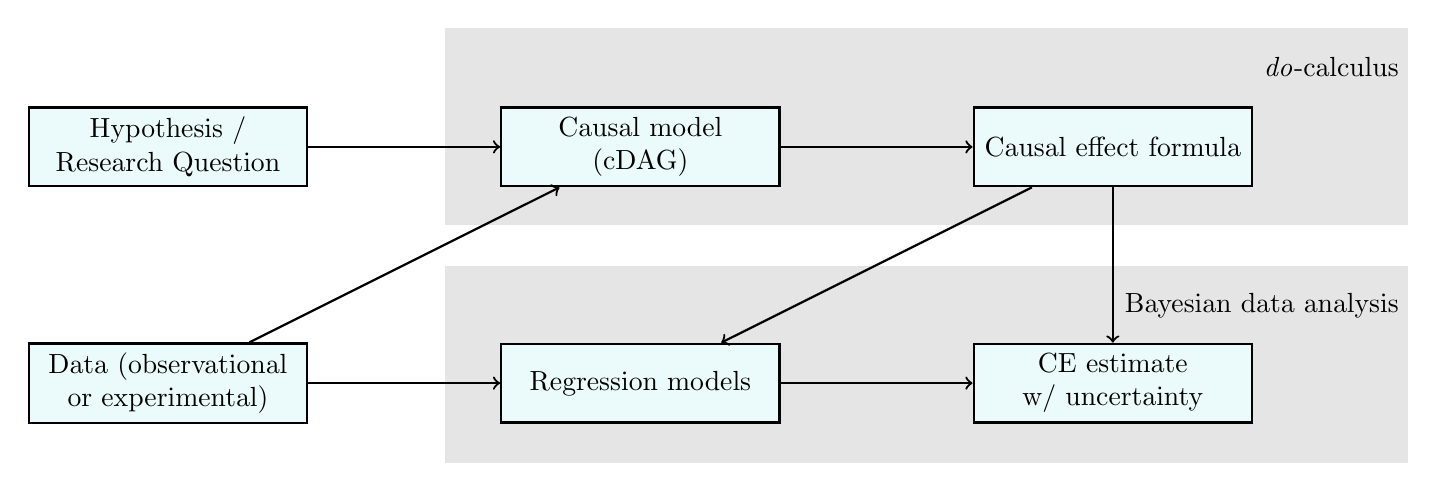
\begin{tikzpicture}[
      node distance=6cm,
      double distance=2pt,
      minimum width=3.5cm,
      minimum height=1cm,
      text centered,
      text width=3.3cm,
      rectangle,
      thick]

      % Background boxes with labels
      \node[fill=gray!20, minimum width=12cm, minimum height=2.5cm, text width=12cm, anchor=south west] (docalc_box) at (3.5,-1) {};
      \node[anchor=north east, text width=5cm, align=right] at (docalc_box.north east) {\docalc};

      \node[fill=gray!20, minimum width=12cm, minimum height=2.5cm, text width=12cm, anchor=north west] (bda_box) at (3.5,-1.5) {};
      \node[anchor=north east, text width=5cm, align=right] at (bda_box.north east) {Bayesian data analysis};

      % NODES
      % anchors
      \node[] (ANCHOR) {};
      % hypothesis
      \node[draw=black, fill=BackgroundR] (hypothesis) {Hypothesis / Research Question};
      % data
      \node[draw=black, fill=BackgroundR, below of = hypothesis, node distance = 3cm] (data) {Data (observational or experimental)};
      % causal inference
      \node[draw=black, fill=BackgroundR, right of = hypothesis] (cdag) {Causal model (cDAG)};
      \node[draw=black, fill=BackgroundR, right of = cdag] (ce) {Causal effect formula};
      % Bayesian data analysis
      \node[draw=black, fill=BackgroundR, right of = data] (bda) {Regression models};
      \node[draw=black, fill=BackgroundR, right of = bda] (result) {CE estimate w/ uncertainty};

      % ARROWS
      \draw[->] (data)--(bda);
      \draw[->] (hypothesis)--(cdag);
      \draw[->] (data)--(cdag);
      \draw[->] (cdag)--(ce);
      \draw[->] (ce)--(bda);
      \draw[->] (ce)--(result);
      \draw[->] (bda)--(result);
    \end{tikzpicture}
  \end{center}

  \caption{Causal effect estimation with the \docalc and Bayesian data analysis.}
  \label{fig:flow-chart}
\end{figure*}

The tutorial is structured as follows.
Section~\ref{sec:experiment} introduces a fictitious data set that will serve as our running example for this tutorial.
The data set instantiates a case of \textit{Simpson's paradox}.
In Section~\ref{sec:theory}, the theoretical background to the \docalc is explained and we use a maximum-likelihood approach to estimate the relevant causal effects for our running example.
Section~\ref{sec:programming} explains how we can obtain estimates of causal effects with quantified uncertainty from Bayesian regression models.
Section~\ref{sec:conclusions--next} reflects what this tutorial achieved and gives references for where to continue learning about causal inference.



\section{Fictitious data \& Simpson's paradox}\label{sec:experiment}

To guide you through the steps of estimating causal effects with the \docalc, we'll look at a concrete numerical example.
Let's assume that we work in a hospital and want to test the effect of a new drug. 
For some reason or other, we cannot simply administer the drug randomly to patients.
Instead, we ask them if they would be willing to test the drug.
In our experiment, we have a random variable (RV) \textsc{drug intake} with two possible values: \textsc{take}, or numerical value $1$, for the participants consenting to test the drug and \textsc{refuse}, or numerical value $0$, for those who declined.
The patients are also sorted into two groups (more on the nature of these groups below).
The concrete numerical data we will work with are shown in Table~\ref{tab:anonymous}.


\begin{margintable}
  \centering
  \begin{tblr}{crcrc}
    \hline
    & \SetCell[c=2]{c} \textsc{refuse}&&\SetCell[c=2]{c}\textsc{take}\\
    \hline
    \textsc{group 1}& $\frac{234}{270}$ & (\textcolor{DarkOrange}{87\%}) & $\frac{81}{87}$ & (\textcolor{DarkGreen}{93\%})\\
    \textsc{group 2}& $\frac{55}{80}$ & (\textcolor{DarkOrange}{68\%}) & $\frac{192}{263}$ & (\textcolor{DarkGreen}{73\%})\\
    $\Sigma$& $\frac{289}{350}$ & (\textcolor{DarkGreen}{83\%}) & $\frac{273}{350}$ & (\textcolor{DarkOrange}{78\%})\\
    \hline
  \end{tblr}
  \caption{Recovery rates after refusing or taking the drug}
  \label{tab:anonymous}
\end{margintable}

\marginnote{The distribution of recovery rates is taken from a real-life medical study \citep{charig1986comparison} and was first discussed in relation to Simpson's Paradox by \citet{julious1994confounding}. The hypothetical experimental setup and the labels of the RVs come from \citet{pearl2000models}.}

How are we to interpret the data in Table~\ref{tab:anonymous} regarding the research question of whether the drug was effective, i.e., whether the rate of recovery increased when taking it?
On the one hand, we see that overall, 83\% of patients who refused the drug recovered from their disease, while only 78\% of the drug-takers did.
This does not bode well for our drug.
However, on the other hand, when we look at each group in isolation, we see that within each group, the drug-takers had a slightly higher recovery rate.
This phenomenon is an instance of \textit{Simpson's Paradox}: Splitting the participants into sub-groups yields different results compared to analyzing all data at once.
This makes the interpretation of our results very difficult: should we use the group-wise results and conclude that the drug is helpful, or should we use the overall results which indicate that the drug is harmful? 
Without further information, specifically on how the groups were formed, we can't take this decision.
This illustrates an important point for statistical analysis: the data alone is not enough to reach conclusions.
The data can't speak for itself. 
We need to be data-literate, so to speak, and bring our knowledge about where the data comes from to bear.

Let's see how adding information about the groups helps our effort to interpret the results. 
We consider two scenarios.
In the first scenario, the participants were grouped by gender (which is treated as a binary variable for the purposes of this example).
\textsc{gender} could be relevant because the drug might have different effects on the male and female body. 
However, \textsc{gender} might also influence the decision to take the drug, e.g., by one gender being more risk averse than the other. 
With the updated group names, the results are displayed in Table \ref{tab:combined}~(a).
A common intuition is that the drug is likely beneficial, because for men and women alike, the chances of recovery are higher for those who took the drug.


Table~\ref{tab:combined}~(b) shows a second scenario for the same numerical values.
Here, the participants were not grouped by gender, but by their blood pressure as measured \textit{after} taking the drug.
Participants are divided into groups with high or low blood pressure. 
In this case, our intuition is likely different. 
Because blood pressure is measured after drug administration and is possibly influenced by the drug, it seems that the groupings into \textsc{high} and \textsc{low} are not as informative, and we should instead focus on the overall results, that tell us that the drug might even be harmful.


\begin{table*}[t]

  \bigskip

  \noindent\rule{\textwidth}{0.4pt}

  \centering

  \begin{subtable}{0.48\textwidth}
    \centering
    \caption{Recovery rates for different genders}
    \label{tab:combined:gender}
    \begin{tblr}{crcrc}
      \hline
      & \SetCell[]{c} \textsc{refuse}&&\SetCell[c=2]{c}\textsc{take}\\
      \hline
      \textsc{men}& $\frac{234}{270}$ & (\textcolor{DarkOrange}{87\%}) & $\frac{81}{87}$ & (\textcolor{DarkGreen}{93\%})\\
      \textsc{women}& $\frac{55}{80}$ & (\textcolor{DarkOrange}{68\%}) & $\frac{192}{263}$ & (\textcolor{DarkGreen}{73\%})\\
      $\Sigma$& $\frac{289}{350}$ & (\textcolor{DarkGreen}{83\%}) & $\frac{273}{350}$ & (\textcolor{DarkOrange}{78\%})\\
      \hline
    \end{tblr}
  \end{subtable}
  %
  \begin{subtable}{0.48\textwidth}
    \caption{Recovery rates for different values of blood pressure}
    \label{tab:combined:bp}
    \centering
    \begin{tblr}{crcrc}
      \hline
      & \SetCell[c=2]{c} \textsc{refuse}&&\SetCell[c=2]{c}\textsc{take}\\
      \hline
      \textsc{low}& $\frac{234}{270}$ & (\textcolor{DarkOrange}{87\%}) & $\frac{81}{87}$ & (\textcolor{DarkGreen}{93\%})\\
      \textsc{high}& $\frac{55}{80}$ & (\textcolor{DarkOrange}{68\%}) & $\frac{192}{263}$ & (\textcolor{DarkGreen}{73\%})\\
      $\Sigma$& $\frac{289}{350}$ & (\textcolor{DarkGreen}{83\%}) & $\frac{273}{350}$ & (\textcolor{DarkOrange}{78\%})\\
      \hline
    \end{tblr}
  \end{subtable}

  \bigskip

  \noindent\rule{\textwidth}{0.4pt}

  \bigskip


  \label{tab:combined}
  \caption{Changing the group names changes our intuitions about the causal effect.}

\end{table*}




\section{Causal inference with the \docalc} \label{sec:theory}

The previous considerations suggest that our intuitions about the correct conclusions to be drawn from experimental data rely on intuitive knowledge of the likely causal role of the relevant measured quantities.
The first step of causal inference is therefore to make such intuitive knowledge explicit (shareable, transparent, open to constructive criticism), e.g., in a formal \textit{causal model}, a version of which is introduced in Section~\ref{sec:causal-models}.
The next step is to determine, based on a causal model, what the effects of \textit{intervening} on a variable would be, as described in Section~\ref{sec:intervention}.
This allows us to specify a formula with which to calculate a notion of causal effect (Section~\ref{sec:causal-effect-formula}), which we can then estimate from the data (Section~\ref{sec:causal-effect}).



\subsection{Causal models} \label{sec:causal-models}

Why do we interpret the data from our two scenarios differently, even though the numbers are exactly the same?
It is because the data is not the only information we have: We also know how this data was obtained and how the variables are most likely related. 
We know that \textsc{gender} ($G$) might have an influence on the decision of \textsc{drug intake} ($D$), while the taking of the drug doesn't change one's gender.
In the case of \textsc{blood pressure} ($B$), we know that it was measured after taking or refusing the drug.
It therefore shouldn't have influenced the decision to take the drug.
However, it is possible that the drug has an influence on blood pressure.
In both cases, we hypothesize that the drug may have an effect on the patients' \textsc{recovery} ($R$).
Before starting with our analysis, we should make these causal relationships explicit.

\begin{marginfigure}

  \centering

  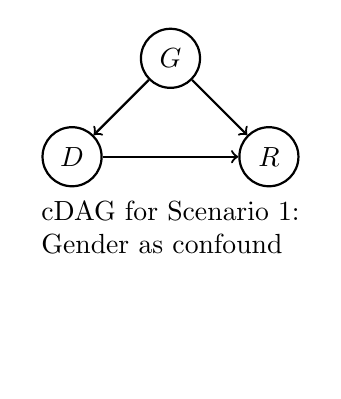
\begin{tikzpicture}[
    node distance = 1.25cm,
    double distance = 2pt,
    minimum size=0.75cm,
    circle,
    thick]
    % NODES
    % anchor
    \node[] (anchor) {};
    % node X
    \node[draw=black, left of = anchor] (D) {$D$};
    % node Y
    \node[draw=black, right of = anchor] (R) {$R$};
    % node Z
    \node[draw=black, above of = anchor] (G) {$G$};
    % caption node
    \node[below of = anchor, align = left, node distance = 0.9cm] (Cap) {cDAG for Scenario 1: \\Gender as confound};

    % ARROWS
    \draw[->] (G)--(D);
    \draw[->] (G)--(R);
    \draw[->] (D)--(R);
  \end{tikzpicture}
  %
  \\ \vspace{-0.5cm}
  %
  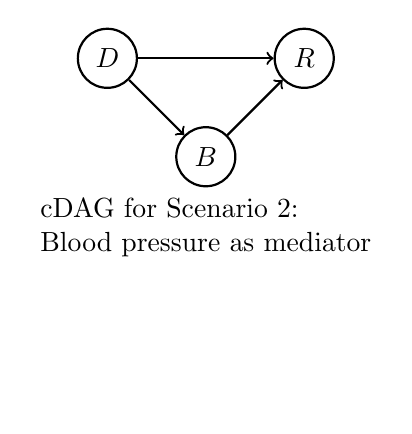
\begin{tikzpicture}[
    node distance = 1.25cm,
    double distance = 2pt,
    minimum size=0.75cm,
    circle,
    thick]
    % NODES
    % anchor
    \node[] (anchor) {};
    % node X
    \node[draw=black, left of = anchor] (D) {$D$};
    % node Y
    \node[draw=black, right of = anchor] (R) {$R$};
    % node Z
    \node[draw=black, below of = anchor] (B) {$B$};
    % caption node
    \node[below of = B, align = left, node distance = 0.9cm] (Cap) {cDAG for Scenario 2: \\Blood pressure as mediator};

    % ARROWS
    \draw[->] (D)--(B);
    \draw[->] (B)--(R);
    \draw[->] (D)--(R);
  \end{tikzpicture}
  %
  \vspace{-1.0cm}
  %
  \caption{Different cDAGs capture our intuitions for different causal roles in the two scenarios.}
  \label{fig:cDAGs-initial}
\end{marginfigure}

One way to make intuitions about causal dependency explicit, is to represent then in a causal model, such as \textit{causal directed acyclic graph} (cDAG).
The nodes in a cDAG represent events, measurements or variables relevant for our data analysis.
We draw an arrow from one node to another to mark the assumption the former is a direct cause of the latter.
The precise details of cDAGs, their relation to causality and stochastic (in-)dependence, are important for advanced applications of causal inference with the \docalc.
As the motivation for this tutorial is to provide a first conceptual feeling of what can be done in this framework, Info Box~1 covers only some of the basics of causal models in a non-technical way.

Figure~\ref{fig:cDAGs-initial} shows the two cDAGs that capture the most common intuitions about causal relations for the two scenarios of Simpson's paradox.
These causal models are considered \textit{a-priori} assumptions about all the relations of direct causation about the variables involved.
\marginnote[-2cm]{The idea of prior knowledge influencing the analysis is familiar to Bayesians.
However, there is one difference: in Bayesian statistics, the influence of the prior over model parameters decreases as the size of the observed data increases.
The \textit{a-priori} causal assumption always influence the outcome.}
Of course, this approach bears some risks.
If we assume the wrong causal relationships, our resulting analysis will also yield wrong results.
However, it is important to note that this is the case for all statistical inference methods.
Any decision on including or excluding a certain variable from statistical analysis is implicitly an assumption about the causal structure connecting the RVs.
Formulating a specific cDAG can thus improve accountability by making the underlying assumptions explicit and easily understandable.

\marginnote{\emph{"All causal inferences based on statistical models are implicitly based on a causal structure"} \citep{shrier2008reducing}}
The construction of a causal model and the question of which variables to include are challenging tasks, especially because in many application cases, the causal structures under observation will be much more complicated than the limited ones given here.
In many cases, it might be impossible to decide between two possible cDAGs.
In these instances, \citet{shrier2008reducing} suggest to perform the analyses on all plausible versions of the DAG.
If the different versions yield different results, all results should be presented. 
In their words: 
\marginnote{From a Bayesian point of view, we can also assign a prior probability to all candidate cDAGs and present, in addition to the estimates of causal effects for each case, a prior-weighted average, similar to other cases of model averaging in Bayesian analysis.}
\begin{quote}
  \emph{Not using the causal approach because of uncertainty on which is the correct DAG simply means that one is allowing chance rather than rational deliberation to make the choice among the different causal diagrams.}
\end{quote}

Once we have settled on one (or several) causal models, the base for our causal analysis is set, and we can continue with the second step: the intervention.

\begin{InfoBox}
\centering
 \colorbox{mygray}{
    \begin{minipage}{1\textwidth}
    \medskip
    \emph{Directed acyclic graphs (DAGs) for causal analysis}
    \medskip

    DAGs can be used to represent causal relationships between \textit{variables}.
    Each variable $X$ can take on any of a set of \textit{values}.
    For example, the variable $D$ for drug-taking can take on values 1 (taken) or 0 (refused).
    The nodes in a causal DAG (cDAG) represent the variables and a directed edge from $X$ to $Y$ indicates that $X$ is a direct cause of $Y$.
    The representation of causal relationships in a cDAG is conventionally interpreted as exhaustive: it contains \textit{all} relations of direct causation; when $X$ and $Y$ are not connected, there is \textit{no} direct causal relation between them.
    % \begin{center}
    %   \begin{tikzpicture}[
    %     node distance = 1.25cm,
    %     double distance = 2pt,
    %     minimum size=0.75cm,
    %     circle,
    %     thick]

    %     %     NODES
    %     %     anchor
    %     \node[] (anchor) {};
    %     %     node X
    %     \node[draw=black, left of = anchor] (X) {$A$};
    %     %     node Y
    %     \node[draw=black, right of = anchor] (Y) {$B$};

    %     %     ARROWS
    %     \draw[->] (A)--(B);
    %   \end{tikzpicture}
    % \end{center}

    A complete assignment of values to each variable is a complete description of the relevant facts, a so-called \textit{world}.
    Causal relations influence the assignment of values to variables either deterministically or probabilistically.
    In \textit{structural equation models} (SEMs), the value of a variable $X$ is completely determined by the set of values assigned to $X$'s direct causes, also called $X$'s \textit{parents}.
    In \textit{probabilistic SEMs}, the value of $X$ is completely determined by two things: (i) as before, the set of values of $X$'s parents, and, additionally, (ii) the value of a stochastic \emph{error variable} $U_{X}$, of which we have one fore each variable in the causal model.
    A special case of probabilistic SEMs are \textit{Bayes Nets} which dispense with the error variables.
    In a Bayes Net each variable $X$ is associated with a probability distribution over $X$'s values, which is a conditional probability for each set of values of $X$'s parents.
    % (Probabilistic SEMs are more expressive than Bayes Nets because they allow error variables to be stochastically dependent, but Bayes Nets can be more intuitive and suffice for many practical applications.)

    By design, probabilistic causal models relate facts about causation to facts about stochastic independence of variables.
    This relationship can be complex, but it can help identify causal structure behind empirical data (\textit{causal discovery}). It can be systematically assessed by decomposing the cDAG's structure into a small number of configurations.
    Two of these, relevant for our running example, are shown below: the chain and the fork.

    \begin{center}
        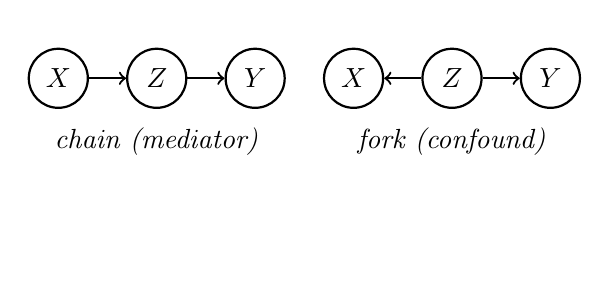
\begin{tikzpicture}[
        node distance = 1.25cm,
        double distance = 2pt,
        minimum size=0.75cm,
        circle,
        thick]

        % NODES
        % anchors
        \node[] (ANCHOR) {};

        \node[draw=black, left of = ANCHOR, node distance = 3.75cm] (anchor_chain) {$Z$};
        \node[below of = ANCHOR, node distance = 0cm] (anchor_fork) {};

        % chain
        \node[draw=black, left of = anchor_chain] (chainX) {$X$};
        \node[draw=black, right of = anchor_chain] (chainY) {$Y$};
        \node[below of = anchor_chain, node distance = 0.8cm] (chain_cap) {\textit{chain (mediator)}};

        % fork
        \node[draw=black, left of = anchor_fork] (forkX) {$X$};
        \node[draw=black, right of = anchor_fork] (forkY) {$Y$};
        \node[draw=black, above of = anchor_fork, node distance = 0cm] (forkZ) {$Z$};
        \node[below of = anchor_fork, node distance = 0.8cm] (fork_cap) {\textit{fork (confound)}};


        % ARROWS
        \draw[->] (chainX)--(anchor_chain);
        \draw[->] (anchor_chain)--(chainY);
        \draw[->] (forkZ)--(forkX);
        \draw[->] (forkZ)--(forkY);
        \end{tikzpicture}
    \end{center}

    \vspace{-1.25cm}
    In a chain, $X$ and $Y$ are causally dependent: $X$ influences the value of the mediator $Z$, which influences $Y$.
    However, $X$ and $Y$ are independent conditioned on $Z$.
    % For example, $X$ could be a drug which influences the blood pressure level $Z$, which influences the likelihood of recovery $Y$.
    % If we know the blood pressure $Z$, additionally learning the value of $X$ (drug or no drug) gives us no further information about the recovery $Y$, as the only way in which the drug influences recovery is through adjusting the level of blood pressure.
    Intuitively put, if $Z$ is a mediator, conditioning on $Z$ undermines the signal about the (indirect) causal influence of $X$ on $Y$.

    In a fork, $Z$ acts as a confound on $X$ and $Y$.
    $X$ and $Y$ are dependent, because they have a common cause in $Z$.
    $X$ and $Y$ become independent conditioned on $Z$.
    % For example, $Z$ could be exercise levels, which influence both weight $X$ and danger of a heart disease $Y$.
    % Knowing $Z$, learning the value of a person's weight $X$ yields no further information on their risk of cardiac disease $Y$.
    Roughly speaking, if $Z$ is a confound, conditioning on $Z$ is necessary to decouple stochastic dependence from information about (indirect) causation.

    For a visual explanation of these causal structures see  \href{https://youtu.be/mBEA7PKDmiY?si=Ihio7ZXJSuct4J30}{{\color{Red}{this lecture}}} by Richard McElreath.
    \medskip
  \end{minipage}
}
\begin{center}
Info Box 2: Background on visually displaying causal relationships.
\end{center}
\end{InfoBox}



\subsection{Intervention} \label{sec:intervention}

The key to inferring causation is intervention.
This is what constitutes the power of the controlled randomized trial setup (if done well) in experimental research.
But what if we cannot, for whatever reason, interfere in the data-generating process?
In that case, we can use our causal model to calculate the effects of a ``simulated intervention'' (this section), which we can use to define how to calculate the causal effect of interest (the next Section~\ref{sec:causal-effect-formula}).
Then, as Pearl has argued prominently, it may be possible to calculate the effects of simulated interventions (and thereby the relevant causal effect) from empirical data from processes that did not involve this intervention (Section~\ref{sec:causal-effect})



% \marginnote{"When we merely observe the value that a variable takes, we are learning about the value of the variable when it is caused in the normal way, as represented in our causal model.
% Information about the value of the variable will also provide us with information about its causes, and about other effects of those causes.
% However, when we intervene, we override the normal causal structure, forcing a variable to take a value it might not have taken if the system were left alone" \citep{sep-causal-models}.}

When we simulate an intervention, we do \textit{as if} we had manipulated the relevant variable, which means that we cut off all influence from upstream causes of that variable, thus possibly creating a modified (pruned, lesioned) cDAG.
We then use the data to estimate the effect that different values of the relevant variable have in this modified cDAG.
In our running example, we want to vary the variable \textsc{drug intake} ($D$), to measure the effects this has on \textsc{recovery} ($R$).
The causal effect of the drug can be estimated by \textit{pretending} that the experimenters had randomly assigned taking or not taking the drug, or placebos to the patients and then comparing the recovery outcomes of the two groups.
In this fictitious scenario, $D$ is the result of random manipulation and thus has no causal ancestors.

Handling such simulated interventions is the main job description of the \docalc. 
The \docalc introduces a new operator, the \doop.
We can now write \doop $\mathdo(D=d)$ to mean that we set the variable $D$ to a fixed value $d \in \{0,1\}$ by intervention.
\marginnote{In the general case, it is also possible to intervene on continuous variables that can take infinitely many values.}
Because the intervention overwrites the normal causal structure, the \doop removes any causal influences on $D$.
In the graphical representation, this means that we can remove any incoming arrows for the variable that we intervene on.
In the cDAG for Scenario 1, $\mathdo(D=d)$ leads to the removal of the causal influence of $G$ on $D$.
In Scenario 2, the \doop has no effect at all, because there were no incoming arrows on $D$ to begin with.
This is illustrated in the updated cDAGs in Figure~\ref{fig:cDAGs-pruned}.

\begin{marginfigure}[1cm]
  \centering
  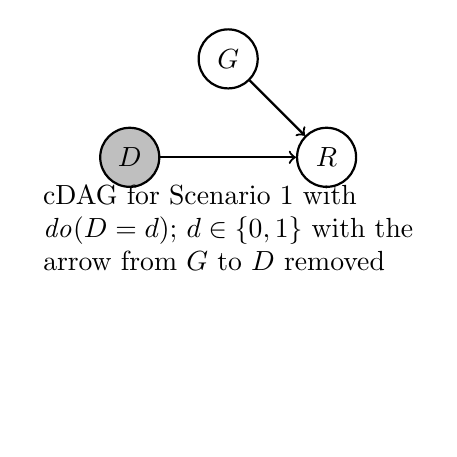
\begin{tikzpicture}[
    node distance = 1.25cm,
    double distance = 2pt,
    minimum size=0.75cm,
    circle,
    thick]
    % NODES
    % anchor
    \node[] (anchor) {};
    % node X
    \node[draw=black, fill=lightgray, left of = anchor] (D) {$D$};
    % node Y
    \node[draw=black, right of = anchor] (R) {$R$};
    % node Z
    \node[draw=black, above of = anchor] (G) {$G$};
    % caption node
    \node[below of = anchor, align = left, node distance = 0.9cm] (Cap) {cDAG for Scenario 1 with\\$\mathdo(D=d)$; $d \in \{0,1\}$ with the\\arrow from $G$ to $D$ removed};

    % ARROWS
    \draw[->] (G)--(R);
    \draw[->] (D)--(R);
  \end{tikzpicture}
  \\
  \vspace{-0.5cm}
  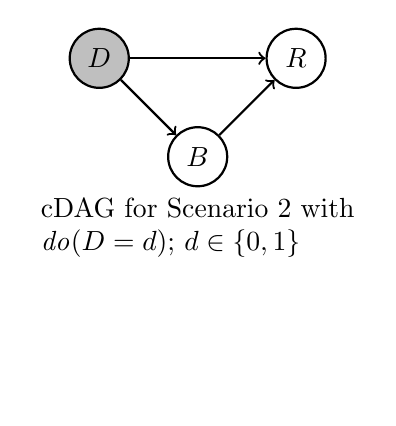
\begin{tikzpicture}[
    node distance = 1.25cm,
    double distance = 2pt,
    minimum size=0.75cm,
    circle,
    thick]
    % NODES
    % anchor
    \node[] (anchor) {};
    % node X
    \node[draw=black, fill=lightgray, left of = anchor] (D) {$D$};
    % node Y
    \node[draw=black, right of = anchor] (R) {$R$};
    % node Z
    \node[draw=black, below of = anchor] (B) {$B$};
    % caption node
    \node[below of = B, align = left, node distance = 0.9cm] (Cap) {cDAG for Scenario 2 with\\$\mathdo(D=d)$; $d \in \{0,1\}$};

    % ARROWS
    \draw[->] (D)--(B);
    \draw[->] (B)--(R);
    \draw[->] (D)--(R);
  \end{tikzpicture}
  \vspace{-1cm}
  \caption{Intervening on a variable in a cDAG amounts to removing all influence from any causally upstream variable.}
  \label{fig:cDAGs-pruned}
\end{marginfigure}

Let's pause here for a second and reflect.
We want to mimic the effects of something like an experimental intervention in a randomized control trial.
The main property that makes such experimental manipulation effective is that the relevant variable (here: $D$) was not allowed to just happen, so to speak.
Some god-like external force (the experimenters) messed up the normal causal flow, interrupted it and just set the variable to whatever they liked, no matter how likely it might have happened on its own had they not intervened on the normal courses of events.
That is, essentially, the main property that makes experimental manipulation potentially informative about causation.
And it is exactly this (cutting off the prior causal influences on the relevant variable ($D$)) that the \docalc implements.
In other words, the \docalc is not some crazy math-voodoo but the most straightforward implementation of what we intuitively consider to be (the power of) systematic experimental manipulation.

\subsection{Causal effect formula} \label{sec:causal-effect-formula}

Given an explicit causal model and a way to represent the idea of an intervention on a variable, we can define what we mean when we speak of a \textit{causal effect}.
Actually, the term ``causal effect'' does not have a single, clear and crisp intuitive meaning.
However, with cDAGs and the \docalc, we can clearly and formally define a number of notions of causal effects.
Here we focus on the most salient notion.
The \textit{average causal effect} of variable $X$ on variable $Y$ is the expected amount of increase of $Y$ given that $X$ is changed (by intervention).
More concretely, for the case of two binary variable such as recovery $R$ and drug use $D$, the average causal effect describes the increase in the probability of recovery $P(R = 1)$ when going from $\mathdo(D=0)$ to $\mathdo(D=1)$, i.e., going from a situation where we intervened so that the drug was \textit{not} given to a situation where we intervened so that the drug \textit{was} given.
In a formula, the average causal effect for our running example is:
\begin{align*}
  \text{Avg-CE}(P \mid D) = & \ P(R=1 \mid \mathdo(D=1)) \  -
                        \\ & \ P(R=1 \mid \mathdo(D=0))
\end{align*}


\subsection{Causal effect estimation} \label{sec:causal-effect}

After defining the causal model to work with and the causal effect of interest, the real challenge arises, namely to calculate the causal effect, if possible, for the given data at hand.
This raises deep conceptual questions:
How do we get from virtual interventions to a causal effect estimation?
And why are we allowed to pretend that an intervention has happened, when the data we have are obtained from a causal process without intervention?
Instead of a general but abstract explanation, the following explores one concrete example of how to obtain a \textit{maximum likelihood estimate} (MLE) of the causal effect in our two scenarios.
In doing so, we explain the mathematical intuition behind why we can (in some cases) treat the data as if it was the product of experimental manipulation.
We look at each scenario in turn.

\paragraph{MLE for Scenario 1: gender as confound.}

As described above, the key to understanding the \docalc is to think of a ``simulated intervention'' as a thought experiment: how would the causal relations be if we had actually intervened on the relevant variable?
In this imagined scenario, we would have seen data generated by a joint probability distribution $\Palt$ over all relevant variables.
Of course, the actual data we have is \textit{not} a sample from $\Palt$, but rather from a joint probability distribution $P$, which follows the dependencies of the assumed cDAG.
So, we would like to use the data, which actually comes from $P$, to estimate ---if possible--- aspects of $\Palt$.
As we said before, sometimes this cannot possibly work; but sometimes it can.
Here is an example of the latter.

Suppose we have data from scenario 1 as in Table \ref{tab:combined}a, which we assume is generated from joint probability distribution $P$.
In the cDAG that (by our working assumption) underlies $P$, variable $D$ was merely observed, not manipulated.
However, we can imagine a case where the joint probability distribution on variables follows $\Palt$ instead, where $D$ was actually experimentally manipulated, so that all upstream causal influences are suppressed.
We now introduce a new piece of notation to write $P\left(R=r \mid \mathdo(D=d)\right)$ for the conditional probability of recovery $R$ given that the drug administration $D$ had been manipulated.
In effect, the conditional probability $P\left(R=r \mid \mathdo(D=d)\right)$ with an imaginary intervention is defined as the conditional probability $\Palt \left(R = r \mid D=d \right)$ under the unobserved probabilities $\Palt$. 
You can think of the \doop as a kind of jumping board to get from the actual probability distribution $P$ to the imagined $\Palt$.
However, this "fictitious" conditional probability cannot always be calculated based on $P$ without further ado, because it assumes that the data-generating process was a different one, namely one that follows the joint distribution $\Palt$.
This makes the \doop seem kind of pointless, like notation juggling or just some renaming trick.
But the good news is that, in some cases, the data obtained from process $P$ can be used to safely estimate all the relevant aspects of $\Palt$, so that we can eventually estimate the desired $P\left(R=r \mid \mathdo(D=d)\right)$ entirely from the non-interventionist data at hand.

As motivated above, by definition we have:
%
\begin{align*}
P\left(R=r \mid \mathdo(D=d)\right) 
& = \Palt \left(R = r \mid D=d \right)
\end{align*}
%
Since the right-hand side of the previous equation has no \doop, the usual rules of probability apply:
%
\begin{align*}
\Palt \left(R = r \mid D=d \right)
& = 
\sum_{g} \Palt \left(R = r \mid D=d, G=g \right) \ \Palt \left( G=g \mid D=d \right)
\end{align*}
%
As variables $D$ and $G$ are stochastically independent in $\Palt$ (see the causal model on the top of Figure~\ref{fig:cDAGs-pruned}), we can simplify:
%
\begin{align*}
& \sum_{g} \Palt \left(R = r \mid D=d, G=g \right) \ \Palt \left( G=g \mid D=d \right) \\
= & \sum_{g} \Palt \left(R = r \mid D=d, G=g \right) \ \Palt \left( G=g \right)
\end{align*}
%
And now the magic unfolds, as we realize that all of the "ingredients" in the last expression, though expressed as probabilities from $\Palt$, can be safely estimated from data generated from $P$, i.e., our actual data.
Why? --- Because we assume that the data-generating processes behind $P$ and $\Palt$ only differ with respect to the dependence of $G$ and $D$, but the remaining (conditional) probabilities, though expressed in $\Palt$, are identical in $P$ (see Figure~\ref{fig:cDAGs-pruned}).
So, we may conclude that, in this particular case, it is possible to "calculate away" the imaginary intervention effect by expressing it entirely in quantities safely estimable from the data at hand, since:
%
\begin{align*}
& \sum_{g} \Palt \left(R = r \mid D=d, G=g \right) \ \Palt \left( G=g \right)
\\
= & 
\sum_{g} P\left(R = r \mid D=d, G=g \right) \ P\left( G=g \right)
\end{align*}
%
The full derivation is repeated more concisely here:
%
\begin{align*}
P&\left(R=r \mid \mathdo(D=d)\right) \\
&= \Palt \left(R = r \mid D=d \right)
& \color{gray}{\text{[by \ def.]}}\\
&= \sum_{g} \Palt \left(R = r \mid D=d, G=g \right) \ \Palt \left( G=g \mid D=d \right)
& \color{gray}{\text{[std. prob.]}}\\
&= \sum_{g} \Palt \left(R = r \mid D=d, G=g \right) \ \Palt \left( G=g \right)
& \color{gray}{\text{[cond. indep.]}}\\
&= \sum_{g} P\left(R = r \mid D=d, G=g \right) \ P\left( G=g \right)
& \color{gray}{\text{[same in $P$]}}
\end{align*}

Now, we can compute the drug's causal effect on recovery by plugging in the numbers from our observational study in Table \ref{tab:combined}.
We compare the recovery rates for cases where the patients took ($P(R=1\mid \do(D=1))$) or refused the drug ($P(R=1 \mid \do(D=0))$):
\begin{equation}
\begin{split}
P(R=1\mid \mathdo(D=1)
&= \sum_{g\in \{0,1\}} P(R=1\mid G=g; D=1) P(G=g)\\
&= \frac{81}{87} \cdot \frac{357}{700} + \frac{192}{263} \cdot \frac{343}{700} \approx 0.83
\end{split}
\end{equation}
\begin{equation}
\begin{split}
P(R=1\mid \mathdo(D=0)
&= \sum_{g\in \{0,1\}} P(R=1\mid G=g; D=0) P(G=g)\\
&= \frac{234}{270} \cdot \frac{357}{700} + \frac{55}{80} \cdot \frac{343}{700} \approx 0.78
\end{split}
\end{equation}
According to these point-valued estimates, patients who take the drug have approximately a 0.83 chance of recovery, while not taking the drug yields a 0.78 chance to recover.
To get the causal effect estimate, we simply have to compare the predicted outcome for patients taking the drug with those refusing it.
The estimated causal effect of \textsc{drug intake} on \textsc{recovery} is thus $P(R=1\mid \mathdo(D=1)-P(R=1\mid \mathdo(D=0) \approx 0.05$, meaning that the drug increases the chance of patients to recover by 5\%.

\paragraph{MLE for Scenario 2: blood pressure as mediator.}

In scenario 2 (see the bottom causal model in Figure~\ref{fig:cDAGs-pruned}), the independent variable $D$ is not causally dependent on any other variable.
The \doop, whose job it is to remove causal influences on the independent variable, thus doesn't have an effect in this case, because there aren't any causal influences on $D$ to begin with.
This means that the observed distribution $P$ is identical to the hypothetical distribution $\Palt$. 
The probability for recovery, in this case, is just $P(R=1\mid D=d)$:
%
\begin{align*}
  P &\left(R=1\mid \mathdo(D=d)\right) \\
    &= \Palt \left(R=1\mid D=d\right)
    & \color{gray}{\text{[by \ def.]}} \\
    &= \sum_{b} \Palt\left(R=1\mid B=b; D=d)\right) \Palt\left(B=b\mid D=d\right)
    & \color{gray}{\text{[std. prob.]}}\\
    &= \sum_{b} P\left(R=1\mid B=b; D=d\right) P\left(B=b\mid D=d\right)
    & \color{gray}{\text{[same in $P$]}}\\
    &= P\left(R=1\mid D=d\right)
\end{align*}

We therefore directly obtain the maximum-likelihood estimates from the \textsc{recovery} frequencies in the data:
\begin{equation}
  \begin{split}
    P(R=1\mid \mathdo(D=1))
    = P(R=1\mid D=1)
    = \frac{273}{350} \approx 0.78
  \end{split}
\end{equation}
%
\begin{equation}
  \begin{split}
    P(R=1\mid \mathdo(D=0))
    = P(R=1\mid D=0)
    = \frac{289}{350} \approx 0.83
  \end{split}
\end{equation}

So, for this case, we estimate that the causal effect of \textsc{drug intake} on \textsc{recovery} is $P(R=1\mid \mathdo(D=\textsc{take})-P(R=1\mid \mathdo(D=\textsc{refuse}) \approx -0.05$.
According to this estimation, taking the drug might actually worsen the chances to recover.
\medskip

Note that while we are able to compute a causal effect estimate by hand using a maximum-likelihood estimation approach, we don't get a measure of certainty without further ado. 
Numerically a causal effect of about 5\% may seem pretty small, so how are we to tell whether this is reliably different from a causal effect size of zero?
This is where the Bayesian approach comes into play.
How to use Bayesian regression modeling to not only estimate causal effects, but quantify uncertainty about these estimates, is the topic of the remainder of this tutorial.

\section{Causal effect estimates from Bayesian Regression} \label{sec:programming}

In this section, we calculate causal effects with Bayesian regression.
Section~\ref{sec:conceptual-approach} first explains \textit{what} it is that we are doing.
Then, Section~\ref{sec:implementation} shows \textit{how} to implement this approach in R using the \texttt{brms} package.

\subsection{Conceptual approach}
\label{sec:conceptual-approach}

As described above, we can compute the causal effect of interest as:
\begin{align*}
  \text{Avg-CE}(R \mid D) & =  P\left(R=1 \mid \mathdo(D=1)\right) - P\left(R=1 \mid \mathdo(D=0)\right)
\end{align*}
In the first scenario, we can reduce the summands on the right-hand side to:
\begin{align*}
  P\left(R=1 \mid \mathdo(D=1)\right) &= \sum_{g} P\left(R = 1 \mid D=1, G=g \right) \ P\left( G=g \right) \\
  P\left(R=1 \mid \mathdo(D=0)\right) &= \sum_{g} P\left(R = 1 \mid D=0, G=g \right) \ P\left( G=g \right)
\end{align*}
In the second scenario, the summands are obtained by:
\begin{align*}
  P\left(R=1 \mid \mathdo(D=1)\right) &= P\left(R=1\mid D=1 \right) \\
  P\left(R=1 \mid \mathdo(D=0)\right) &= P\left(R=1\mid D=0 \right)
\end{align*}
Taken together, we need estimates of three types of probabilities:
\begin{itemize}
  \item the unconditional probability $P(G=g)$ for gender categories
  \item the conditional probability $P(R=1 \mid D=d, G=g)$ of recovery given $D$ and $G$
  \item the conditional probability $P(R=1 \mid D=d)$ of recovery given $D$
\end{itemize}
We, as modellers, are uncertain about these probabilities, but the available data let's us estimate each.
The MLE from the previous section demonstrated this, but these estimates did not (directly) express the amount of uncertainty we have.
To resolve this, we are going to use Bayesian regression modeling to estimate these probabilities, using the usual sampling-based approach.
Samples for the relevant (conditional and unconditional) probabilities involved will then contain information about how certain we are about our estimates.

To understand how regression comes in, you need to understand a few crucial, general aspects.
\begin{enumerate}[1.]

  \item A conditional probability distribution like $P(Y \mid X_{1}, \dots, X_{n})$ can be approximated with a regression model which we would normally specify with R's formula syntax: $Y \sim X_{1} * \dots * X_{n}$.
  If we want to estimate an unconditional probability $P(Y)$, we can do so with a so-called ``intercept-only'' model, as given by regression formula: $Y \sim 1$.

  \item For our current purposes, where we are dealing with binary variables, we need to look at logistic regression models.

  \item Logistic regression models, like other generalized regression models, make predictions at different levels for any value of predictive variables $X_{1}, \dots, X_{n}$.
  \marginnote{In (non-generalized) standard regression models, the linear predictor and the central tendency are the same.}
  They predict values for
  \begin{enumerate}[(i)]
    \item the linear predictor,
    \item the central tendency, and
    \item the dependent / response variable $Y$.
  \end{enumerate}

  \item Since we are dealing with binary variables and logistic regression, what we care about are predictions at the second level, the level of central tendency.
  Concretely, we want an estimate of a probability like $P(G=1)$, which is the probability of a participant being male.
  That's a prediction of central tendency.
  We do not want a prediction of a log-odds ratio (the linear predictor) or prediction of a single binary category (male or female).
  \marginnote[-2cm]{We can obtain a prediction of central tendency by sampling many concrete values of the response variable, but that is less efficient than sampling a value of central tendency directly.}

  \item In a Bayesian regression model all of these predictions are probabilistic, since they represent our uncertainty about these values (as we estimate them from limited data).
  In a usual Bayesian workflow, we would therefore obtain samples from the so-called \textit{posterior predictive distribution} for each one of these different levels.
  \marginnote[-1.7cm]{For a detailed explanation of the differences of drawing samples from different levels of posterior predictive distributions, see \href{https://www.andrewheiss.com/blog/2022/09/26/guide-visualizing-types-posteriors/}{{\color{Red}{this blog post}}}.}

\end{enumerate}

These points taken together yield the following approach.
We use logistic regression with the appropriate dependent and independent variables to get at the relevant conditional or unconditional probabilities.
We use samples from the posterior predictive distribution of central tendency (the category probabilities).
For scenario one, we need to do this in a nested fashion, to reflect the causal effect formula for this case.
Our uncertainty about the causal effect estimate is the propagated uncertainty inherent in the samples from the posterior predictive distribution.


\subsection{Implementation}
\label{sec:implementation}

Having established the conceptual basics, let's now dive into the programming part.
%
\marginnote{The entire code is available at \href{https://github.com/michael-franke/BayesReg-CausalInference}{{\texttt{https://github.com/michael-franke/\\BayesReg-CausalInference}}}.}
%
First, we set up the environment and load the required packages:
%
\begin{minipage}[]{\textwidth}
\begin{lstlisting}[language=R]
#### packages, options, seed ----

# for Bayesian regression modelling
library(brms)       # Bayesian regression models
library(HDInterval) # for calculating highest density intervals
library(tidybayes)  # for tidy output of Bayesian models
# for data wrangling
library(tibble)     # dataframes
library(tidyr)      # for tidying dataframes
library(dplyr)      # intuitive data manipulation
# for plotting
library(ggplot2)    # for plots

# option for Bayesian regression models:
# use all available cores for parallel computing
options(mc.cores = parallel::detectCores())

# seeding for reproducibility
set.seed(123)
\end{lstlisting}
\end{minipage}

\vspace{-0.5cm}
We also the number of samples to use for each variable:

\begin{minipage}[]{\textwidth}
\begin{lstlisting}[language=R]
# global parameter: number of iterations / samples
n_iter = 5000
\end{lstlisting}
\end{minipage}

\vspace{-0.5cm}
Next, we create a dataset with the values from Table \ref{tab:combined} and transform it into the required shape.

\begin{minipage}[]{\textwidth}
\begin{lstlisting}[language=R]
#### preparing the data set ----

# generate dataset with Simpsons paradox
data_simpsons_paradox <- tibble(
  gender = c("Male", "Male", "Female", "Female"),
  bloodP = c("Low", "Low", "High", "High"),
  drug = c("Take", "Refuse", "Take", "Refuse"),
  k = c(81, 234, 192, 55),
  N = c(87, 270, 263, 80),
  proportion = k/N
)

# cast into long format (one observation per row)
data_SP_long <- rbind(
  data_simpsons_paradox |>
    uncount(k) |>
    mutate(recover = TRUE) |>
    select(-N, -proportion),
  data_simpsons_paradox |>
    uncount(N-k) |>
    mutate(recover=FALSE) |>
    select(-k, -N, -proportion)
  ) |> # this part is new
  mutate(
    gender = factor(gender),
    drug = factor(drug)
  )
\end{lstlisting}
\end{minipage}

\vspace{-0.5cm}
Now, we can start modeling!

\paragraph{Scenario 1: Gender as confound.}
In scenario 1, the effectiveness of the drug is confounded by \textsc{gender}.
As described above, we need to model two probability distributions:
the (unconditional) probability of \textsc{gender}, $P\left( G=g \right)$ and
the (conditional) probability of \textsc{recovery}, $P\left(R = r \mid D=d, G=g \right)$.
Therefore, we first fit an intercept-only regression model which allows us to estimate the distribution of \textsc{gender}, $P\left( G=g \right)$.

\begin{minipage}[]{\textwidth}
\begin{lstlisting}[language=R]
# estimate the distribution of gender
#   (by intercept-only regression)
fit_gender <- brm(
  formula = gender ~ 1,
  data = data_SP_long,
  family = bernoulli(link = "logit"),
  iter = n_iter
)
\end{lstlisting}
\end{minipage}

\vspace{-0.5cm}

Next, we fit a regression model to help estimate the conditional probability of recovery, $P\left(R = r \mid D=d, G=g \right)$.

\begin{minipage}[]{\textwidth}
\begin{lstlisting}[language=R]
# estimate the distribution of recovery rates as predicted
#   by gender and treatment
fit_recovery_gender <- brm(
  formula = recover ~ gender * drug,
  data = data_SP_long,
  family = bernoulli(link = "logit"),
  iter = n_iter
)
\end{lstlisting}
\end{minipage}

To get samples from the posterior predictive distributions (of central tendency) of fitted models, we use the function \ri{epred\_draws()} from the \textit{tidybayes} package.
\marginnote{Notice that the variance in these samples is what quantifies our (modeller's) uncertainty about the value $P(G=1)$.}
For the case at hand, since we want samples of $P(G=1)$, we pass the intercept value of 1 in the \ri{newdata} argument of the \ri{epred\_draws()} function.
Each sample from the posterior predictive distribution of central tendency is a probability value between 0 and 1, which we can interpret as the estimated fraction of men in the sample.

\begin{minipage}[]{\textwidth}
\begin{lstlisting}[language=R]
#  estimate gender distribution by sampling from the expected value
#    of the posterior predictive distribution
#  (estimate the fraction of men in the sample)
posterior_gender_proportion <- tidybayes::epred_draws(
  object = fit_gender,
  newdata = tibble(Intercept = 1),
  value = "maleProp", #proportion of men in the sample
  ndraws = n_iter * 2
) |> ungroup() |>
  select(.draw, maleProp)
\end{lstlisting}
\end{minipage}

\vspace{-0.5cm}
We then estimate the average recovery rate for all combinations of \textsc{gender} and \textsc{drug intake} by drawing from the expected values of the posterior predictive distributions of the \textsc{recovery} regression model.
To do so, we first define a data structure with all combinations of levels of the predictor variables.

\begin{minipage}[]{\textwidth}
\begin{lstlisting}[language=R]
# make a data frame with all compbinations of values for variables
#   of drug and gender
newdata <- tibble(
  gender = factor(c("Male", "Male", "Female", "Female"), levels = levels(data_SP_long$gender)),
  drug = factor(c("Take", "Refuse", "Take", "Refuse"), levels = levels(data_SP_long$drug))
)
\end{lstlisting}
\end{minipage}

\vspace{-0.5cm}
This structure is passed into the argument \ri{newdata} to obtain samples from the posterior predictive distribution of central tendency, via \ri{epred\_draws()} as before.

\begin{minipage}[]{\textwidth}
\begin{lstlisting}[language=R]
# get posterior predictive samples for each combination of values
#  for drug and genders
posterior_g <- tidybayes::epred_draws(
  object  = fit_recovery_gender,
  newdata = newdata,
  value   = "recovery",
  ndraws  = n_iter * 2
) |> ungroup() |>
  select(.draw, gender, drug, recovery)
\end{lstlisting}
\end{minipage}

\vspace{-0.5cm}
The data frame \ri{posterior_g} now contains samples of $P(R=1 \mid D=d, G=g)$.
We need to multiply each prediction for $P(R=1 \mid D=d, G=g)$ with a sample of $P(G=g)$, the estimated fraction of men and women, respectively, which are stored in \ri{posterior_gender_proportion}.
This allows us to obtain samples of the causal effect we are interested in.

\begin{minipage}[]{\textwidth}
\begin{lstlisting}[language=R]
# obtain estimates of causal effect by
#   calculating the weighted average of recovery rates for each
#   value of drug, weighted by the est. proportions of males
posterior_g <- posterior_g |>
  # add the previous samples of P(G=1)
  #  and flip, where necessary, to P(G = 0)
  full_join(posterior_gender_proportion) |>
  mutate(weights = ifelse(gender == "Male",
                          maleProp, 1-maleProp)) |>
  # calculate P(G=g) * P(R|G=g, D=d) for each combination of G and D
  group_by(`.draw`, drug) |>
  summarize(predRecover = sum(recovery * weights)) |>
  pivot_wider(names_from = drug, values_from = predRecover) |>
  # causal effect estimates are obtained from by subtracting
  #   the predicted recovery rates when the drug is refused from
  #   the predicted recovery rates when the drug is taken
  mutate(causal_effect = Take - Refuse)
\end{lstlisting}
\end{minipage}

\vspace{-0.5cm}
The results of these computations are summarized with the \ri{summarize_posterior} function:
  \marginnote{\texttt{summarize\_posterior} is a custom helper function. You can find it on the \href{https://github.com/michael-franke/BayesReg-CausalInference}{{\color{Red}{GitHub page}}} of this tutorial.}

\begin{minipage}[]{\textwidth}
\begin{rc}
> summarize_posterior(posterior_DrugRefused_g,
                      posterior_DrugTaken_g)
# A tibble: 3 x 4
  condition     CI_lower   mean CI_upper
  <fct>            <dbl>  <dbl>    <dbl>
1 take drug       0.792  0.832     0.869
2 refuse drug     0.726  0.778     0.834
3 causal effect  -0.0121 0.0534    0.120
\end{rc}
\end{minipage}

\vspace{-0.5cm}
Similar to the MLE approach, we obtain a causal effect estimate of about 5\%, i.e., patients are predicted to have a roughly 5\% higher chance of recovery when taking the drug.
However, we can see that the credible interval includes 0, which suggests that we do not have enough evidence to rule out that the drug has no causal effect.

\paragraph{Scenario 2: Blood pressure as mediator}
In scenario 2, blood pressure acts as a mediator between the drug and the patients’ recovery.
As described above, we simply need to calculate the conditional recovery probability $P(R=1 \mid D=d)$.
Therefore, we fit \textsc{recovery} to \textsc{drug intake}.

\begin{minipage}[]{\textwidth}
\begin{lstlisting}[language=R]
# fitting a regression model to predict recovery based on drug use alone
fit_recovery_bp <- brm(
  formula = recover ~ drug,
  data = data_SP_long,
  family = bernoulli(link = "logit"),
  iter = n_iter
)
\end{lstlisting}
\end{minipage}

\vspace{-0.5cm}
As we do not have to do any further calculations to estimate the causal effect in scenario 2, all we need to do is extract the relevant posterior predictive samples, and computing samples of the causal effect, as we did previously.

\begin{minipage}[]{\textwidth}
\begin{lstlisting}[language=R]
# posterior predictive samples for the recovery rate
#   when the drug is refused and taken
posterior_bp <-
  tidybayes::epred_draws(
    object = fit_recovery_bp,
    newdata = tibble(drug = c("Refuse", "Take")),
    value = "predRecover", # prob. of recovery
    ndraws = n_iter * 2
  ) |> ungroup() |>
  select(.draw, drug, predRecover) |>
  pivot_wider(names_from = drug, values_from = predRecover) |>
  # causal effect estimates are obtained from by subtracting
  #   the predicted recovery rates when the drug is refused from
  #   the predicted recovery rates when the drug is taken
  mutate(causal_effect = Take - Refuse)
\end{lstlisting}
\end{minipage}

\vspace{-0.5cm}
Summary statistic for these samples of causal effect estimates are:

\begin{minipage}[]{\textwidth}
\begin{rc}
> summarize_posterior(posterior_DrugRefused_bp, posterior_DrugTaken_bp)
# A tibble: 3 x 4
  condition     CI_lower    mean CI_upper
  <fct>            <dbl>   <dbl>    <dbl>
1 take drug        0.736  0.779    0.823
2 refuse drug      0.785  0.825    0.863
3 causal effect   -0.103 -0.0458   0.0131
\end{rc}
\end{minipage}

\vspace{-0.5cm}
We can see that taking the drug yields an estimated 78\% chance of recovery, while not taking it leads to a 83\% chance.
The causal effect is estimated to be -5\%, such that taking the drug is estimated to have detrimental effects on recovery.
As in the first scenario, the CI includes 0, so that we cannot safely rule out that there is no causal effect.

\begin{figure}
    \centering
    \includegraphics[width=0.8\linewidth]{../code/posterior_causal_effect_smooth.png}
    \caption{Posterior distributions of the causal effect for both scenarios. Bold Black lines indicate 95\% credible intervals, the posterior means are shown as black dots.}
    \label{fig:posteriors}
\end{figure}

\section{Conclusions \& next steps}
\label{sec:conclusions--next}

Taking a step back, what can we learn from these hypothetical scenarios?
The data for both scenarios was identical.
Despite that, the computations of causal effects were different and the results reflected this: even though both causal effects were not credibly different from zero, they point in different directions, as can be seen in Figure \ref{fig:posteriors}.
This illustrates the importance of choosing the correct causal structure. 
Going beyond our hypothetical scenarios, we showed that the \docalc can, in some scenarios, be used to estimate causal effects, even if the data at hand stems from observational studies.
To estimate the causal effects, both frequentist (MLE) and Bayesian methods yield similar results, yet only with a Bayesian sampling-based approach also allowed us to flexibly quantify the uncertainty of causal effect estimates.

\begin{InfoBox}
\centering
\colorbox{mygray}{
  \centering
  \begin{minipage}{1\textwidth}
    \medskip

    \emph{The Neyman-Rubin Causal Model / potential outcome framework}
    \medskip

    The Neyman-Rubin causal model is based on the framework of potential outcomes that a treatment would have on an individual.
    As an example, let's consider going to college as the treatment, and future income as the outcome of interest.
    The causal effect of going to college on the individual's future income is defined as the difference between the income with and without a college degree.
    This notion of causal effect is a hypothetical measure, as the potential outcomes are counterfactual and only one of them can be observed.
    Importantly, the potential outcomes are treated as fixed quantities and not random variables.
    This is different from \docalc, where the outcomes are also stochastic, and the assignment of treatment is fixed/deterministic.
    The only stochastic process in the Neyman-Rubin causal model is the assignment of treatment, which depends on the observable characteristics $X$.
    These could, for example, be high school grades, socio-economic background or gender.
    Because the potential outcomes are fixed, any two individuals who share the same set of characteristics $X$ have the same potential outcomes.
    This can be leveraged to compute the causal effect.
    For each combination of values $X$ can take, the income of individuals who went to college can be compared with that of those who didn't.
    This procedure is called matching.
    Because it is in most cases not easy to find individuals with exactly matching values of $X$, especially for continuous variables, there are different proposed matching methods \citep{sekhon2008neyman}.

    \medskip

    \emph{Structural Equation Modeling}
    \medskip

    A structural equation model (SEM) is a causal model that combines observable and latent variables.
    The causal connections between variables are represented with equations and treated as a-priori.
    SEMs can also be represented graphically in path diagrams.
    A path diagram is not the same as a cDAG, because it is not acyclic and can involve feedback relations. However, in this case, the model is underidentified and non-testable.
    The goal of a SEM is to estimate the values of latent variables from the measured values of the observable variables.
    SEMs can be evaluated with measures of model fit.
    In case of a bad fit, the causal assumptions underlying model formulation can be regarded as falsified \citep{bollen2013eight}.

    It has been shown that the potential outcome framework and structural equation modeling are logically equivalent \citep{galles1998axiomatic, halpern2000axiomatizing}.
    \citet{pearl2000models} combined features of the potential outcome framework and SEM to formulate the structural causal model as a general theory of causation.

    \medskip


  \end{minipage}
}
\begin{center}
Info Box 1: Alternatives to the \docalc for causal inference.
\end{center}
\end{InfoBox}



\printbibliography[heading=bibintoc]

\end{document}
